\documentclass[40pt,twoside,a4paper]{article}
% http://www-h.eng.cam.ac.uk/help/tpl/textprocessing/latex_maths+pix/node6.html symboles de math
% http://fr.wikibooks.org/wiki/Programmation_LaTeX Programmation latex (wikibook)
%=========================== En-Tete =================================
%--- Insertion de paquetages (optionnel) ---
\usepackage[french]{babel}
\usepackage{a4}	             % pour la taille   
\usepackage[T1]{fontenc}     % pour les font postscript
\usepackage{epsfig}          % pour gerer les images
%\usepackage{psfig}
\usepackage{amsmath, amsthm} % tres bon mode mathematique
\usepackage{amsfonts,amssymb}% permet la definition des ensembles
\usepackage{float}           % pour le placement des figure
\usepackage{verbatim}
\usepackage{longtable} % pour les tableaux de plusieurs pages
\usepackage[table]{xcolor} % couleur de fond des cellules de tableaux
\usepackage{lastpage}
\usepackage{multirow}
\usepackage{multicol} % pour {\'e}crire dans certaines zones en colonnes : \begin{multicols}{nb colonnes}...\end{multicols} 

% \usepackage[top=1.5cm, bottom=1.5cm, left=1.5cm, right=1.5cm]{geometry}
% gauche, haut, droite, bas, entete, ente2txt, pied, txt2pied
\usepackage{vmargin}
\setmarginsrb{1.0cm}{1.0cm}{1.0cm}{1.0cm}{22pt}{3pt}{60pt}{25pt}

\usepackage{lscape} % changement orientation page
%\usepackage{frbib} % enlever pour obtenir references en anglais
% --- style de page (pour les en-tete) ---
\pagestyle{headings}


\def\logoCreativeCommon{img/CreativeCommonLogo.jpeg}
\def\includeLogoCC{\includegraphics[width=0.25cm]{\logoCreativeCommon }}
\def\MainTitle{Cyber Age / Cyberpunk -- Geekopolis 2014 -- \emph{AmaelAssour} \includegraphics[width=0.30cm]{\logoCreativeCommon } \today }

% mettre du texte en diagonale sur le fond : tikz
\usepackage{tikz} 
\def\confidentialTIKZ{%
	\begin{tikzpicture}[remember picture,overlay]
	\node[rotate=60,scale=15,text opacity=0.2] at (current page.center) {Confidentiel};
	\end{tikzpicture}
}%

\def\confidentialDGTIKZ{%
	\begin{tikzpicture}[remember picture,overlay]
	\node[rotate=60,scale=7.5,text opacity=0.2] at (current page.center) {Confidential -- Delta Green};
	\end{tikzpicture}
}%

\def\confidentialDGopeFallAngelsTIKZ{%
	\begin{tikzpicture}[remember picture,overlay]
	\node[rotate=60,scale=5.5,text opacity=0.2] at (current page.center) 
		{DG Restreint -- Op. Fallen Angels}; %%  Op{\'e}ration Fallen Angels
	\end{tikzpicture}
}%

\def\cyberAge2080TIKZ{%
	\begin{tikzpicture}[remember picture,overlay]
	\node[rotate=60,scale=7.5,text opacity=0.2] at (current page.center) {Cyber Age -- Cyberpunk 2080};
	\end{tikzpicture}
}%

% % % en-tete et pieds de page configurables : fancyhdr.sty
% http://www.trustonme.net/didactels/250.html
% http://ww3.ac-poitiers.fr/math/tex/pratique/entete/entete.htm
% http://www.ctan.org/tex-archive/macros/latex/contrib/fancyhdr/fancyhdr.pdf
\usepackage{fancyhdr}
\pagestyle{fancy}
% \newcommand{\chaptermark}[1]{\markboth{#1}{}}
% \newcommand{\sectionmark}[1]{\markright{\thesection\ #1}}
\fancyhf{}
\fancyhead[LE,RO]{
	\cyberAge2080TIKZ
	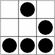
\includegraphics[width=0.5cm]{img/logo_glider.png} 
	\hfill \MainTitle \hfill
	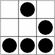
\includegraphics[width=0.5cm]{img/logo_glider.png} 
	} %% {\bfseries\thepage}
\fancyfoot[LE,RO]{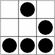
\includegraphics[width=0.5cm]{img/logo_glider.png} 
	\hfill \MainTitle \hfill
	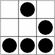
\includegraphics[width=0.5cm]{img/logo_glider.png} } %% {\bfseries\thepage}
%% \fancyhead[LO]{\bfseries\rightmark}
%% \fancyhead[RE]{\bfseries\leftmark}
%% \fancyfoot[LE]{\thepage /\pageref{LastPage} \hfill
%% 	\MainTitle 
%% \hfill 
\includegraphics[width=0.5cm]{img/DeltaGreenLogo.png} }
%% \fancyfoot[RO]{
\includegraphics[width=0.5cm]{img/DeltaGreenLogo.png} \hfill
%% 	\MainTitle 
%% \hfill \thepage /\pageref{LastPage}}
\renewcommand{\headrulewidth}{0.25pt}
\renewcommand{\footrulewidth}{0.50pt}
\addtolength{\headheight}{0.5pt}
\fancypagestyle{plain}{
	\fancyhead{}
	\renewcommand{\headrulewidth}{0pt}
}

%--- Definitions de nouvelles commandes ---
\newcommand{\N}{\mathbb{N}} % les entiers naturels

%--- Definitions de nouvelles couleurs ---
\definecolor{verylightgrey}{rgb}{0.8,0.8,0.8}
\definecolor{verylightgray}{gray}{0.80}
\definecolor{lightgrey}{rgb}{0.6,0.6,0.6}
\definecolor{lightgray}{gray}{0.6}

%============================= Corps =================================
\begin{document}

\setlength\parindent{0pt}

%% \confidentialDGTIKZ

\begin{center} 
	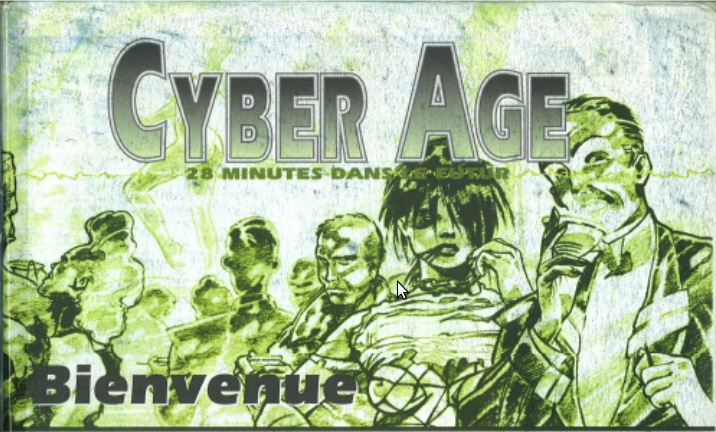
\includegraphics[width=0.90\textwidth]{img/CyberAgeBienvenue.jpeg} %\hfill
\end{center}

\begin{minipage}[ht]{0.15\textwidth}
	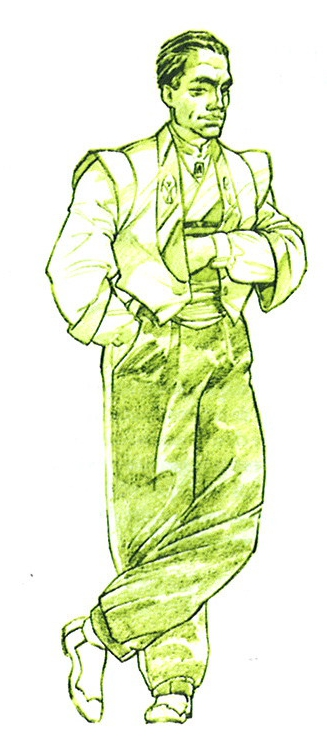
\includegraphics[width=0.95\textwidth]{img/personnagePaulMorgan.jpg} ~\\~\\
	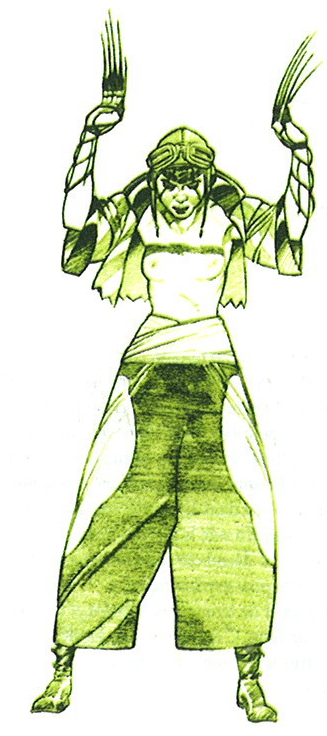
\includegraphics[width=0.95\textwidth]{img/personnageIrinaToss.jpg} ~\\~\\
\end{minipage} \hfill \begin{minipage}[ht]{0.65\textwidth}
	\textbf{\LARGE Cyber Age -- Explorez les ann{\'e}es 2080 !} ~\\~\\
	
	\begin{center}
		\textsc{\LARGE Connectez-vous {\`a} HyperNet !~\\ 
			$\Longrightarrow$ Le cyberespace en 3D ! $\Longleftarrow$}
	\end{center}
	~\\~\\
	
	\textsc{\LARGE Visitez les Jungles Urbaines !}~\\~\\
	\textsc{\LARGE Investissez dans les {\^I}les de la Lune !}~\\~\\
	
	{\Large
		Bienvenue dans les ann{\'e}es 2080 : un univers de folie cybern{\'e}tique o{\`u} la conqu{\^e}te spatiale est devenue r{\'e}alit{\'e} !~\\~\\
		Le cyberespace est {\'e}galement de la partie : la virtualit{\'e} est d{\'e}sormais r{\'e}alit{\'e} !~\\~\\
		Visitez des centres urbains de qualit{\'e} avec des moyens de transport ultr-rapides terrestres a{\'e}riens et spatiaux !~\\~\\
		Assistez en direct {\`a} une guerre priv{\'e}e entre M{\'e}ga-Corporations !~\\~\\
		Faites un Tour dans une Arcologie de Euro/Matsushita : Nouvelle Babylone !~\\~\\
	}

\end{minipage} \hfill \begin{minipage}[ht]{0.15\textwidth}
	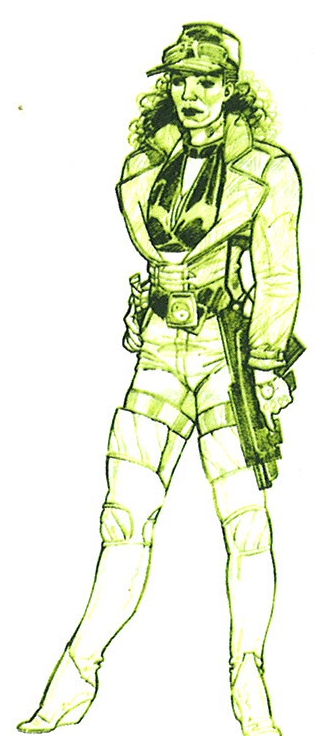
\includegraphics[width=0.95\textwidth]{img/personnageSandraVitteker.jpg} ~\\~\\
	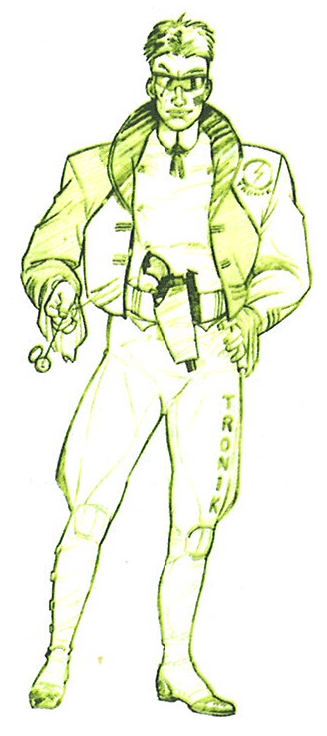
\includegraphics[width=0.95\textwidth]{img/personnageJeremiahSteel.jpg} ~\\~\\
\end{minipage} ~\\

\hrule



\hrule

~\\

\end{document}
